\addchap{Irgendwie, Irgendwo, Irgendwann}

\begin{wrapfigure}[6]{r}{0.2\textwidth}
  \vspace*{-11pt}
  \textcolor{KIFgrey}{\qrcode[height=.2\textwidth]{https://navigator.tu-dresden.de}}
\end{wrapfigure}

Man kann die \KIF{} aufgrund der zurückzulegeden Wege zwischen relevanten Orten auch als eine \enquote{MiniKIF} bezeichnen. Dennoch erstreckt sie sich über mehr als ein Gebäude.
Für den Fall, dass ihr euch des Weges von A nach B einmal nicht sicher seid, oder ihr ein Faible für digitale Raumpläne und Karten habt, könnt ihr euch den Campusnavigator für Android \link{https://play.google.com/store/apps/details?id=de.tud.campusnavigator} oder iOS \link{https://itunes.apple.com/de/app/campus-navigator-tu-dresden/id722282377} herunterladen und mit dem nebenstehenden QR-Code direkt zum Andreas-Pfitzmann-Bau springen.

\section*{Die Informatikfakultät -- Andreas-Pfitzmann-Bau}
Im Andreas-Pfitzman-Bau (APB) ist die hiesige Informatikfakultät und wird euer Hauptaufenthaltsort während der \KIF{}.
Bitte beachtet, dass im gesamten Gebäude (wie auch in allen anderen Campusgebäuden) Rauchverbot herrscht.
Der Rest der Hausordnung fällt in die Kategorie \enquote{gesunder Menschenverstand}, sollte also niemanden einschränken.
Um innerhalb dieses Gebäudes die relevanten Räumlichkeiten besser finden zu können, haben wir für euch ein schilderbasiertes Leitsystem im Gebäude installiert.
Folgt ihr den richtigen Schildern, kommt ihr also auch ans richtige Ziel.

\subsection*{Der Teich}
Im inneren Außenbereich der Fakultät könnt ihr euch am Teich entspannen und das hoffentlich schöne Wetter genießen.
Beachtet aber, dass der Teich von Fischen und ähnlichen Lebewesen mit Kiemen bewohnt wird.
Neueste Erkenntnisse zeigen, dass Menschen nicht in diese Kategorie fallen.

\subsection*{Infopoint -- E017}
Der zweite Teil der Eskalationshierarchie führt euch bei Fragen oder Problemen zum Infopoint.
Wir haben unser FSR-Büro so umgebaut, dass dieses einen 20 Köpfigen Mob fragender KIFfel gleichzeit aufnehmen und auf Antworten warten lassen kann.
Die E017 befindet sich versteckt aber doch vorhanden hinter der Wendeltreppe und wird in diesen Tagen vermutlich das erste Mal nicht ausschließlich zur Prokrastination genutzt.
Scheut euch nicht eure Fragen vorzubringen, denn die hier eingeteilten Engel werden ihr möglichstes Tun, euch weiterzuhelfen.

\subsection*{KIF-Café -- E023}
Der einzige im Andreas-Pfitzmann-Bau befindliche Hörsaal wurde von uns mithilfe eurer Einsedungen zum KIF-Café Umdekoriert.
Da die Schlafhallen und Seminarräume zeitunabhängig benutzbar sein werden, gibt es kein dediziertes ruhiges KIF-Café.
Die E023 ist also zentraler Treffpunkt und Aufenthaltsraum und steht für Austausch, Spiel und Spaß jederzeit zur Verfügung.
Die aufgebauten Sofas sollen als gemütliche \textbf{Sitzplätze} genutzt werden.
Entscheided euch also bei Müdigkeit lieber für die Schlafhalle.
Andere KIFfel werden es euch danken.

\subsection*{Ewiges Frühstück -- E008}
Die wichtigste Mahlzeit einer jeden KIF ist bei uns in einem Seminarraum erhältlich.
Das Ewige Frühstück befindet sich nicht weit vom KIF-Café entfernt im Raum mit der Nummer 8.
Da das KIF-Café der einzige von uns genutze Raum mit mehr als einem Zugang ist, solltet ihr darauf achten, dass die Tür zum Ewigen Frühstück für einen Besseren Menschenfluss immer Freigehalten wird.
Versucht also für etwaige Warteschlangen den Platz im Raum selbst zu nutzen.
Sollten euch Mängel in jeglicher Hinsicht und zu jeglicher Zeit auffallen, zögert nicht, es den eingeteilten Frühstücksengeln mitzuteilen.

\subsection*{AK Tee -- E007}
Eine in Bremen erstmalig angewandte Methode wird nach der Fortführung in Frankfurt letztendlich in Dresden durch ihr drittes Auftreten zur Tradition.
Ein dauerhafter Arbeitskreis mit der Bezeichnung \enquote{Tee} bekommt einen dedizierten Raum: E007.
Setzt euch dazu und trinkt Tee.
Gerade in diesem Raum sollte ein einem Arbeitskreis gerechter Geräuschpegel herrschen.
% TODO: 1,5 Zeilen mehr Tee.

\subsection*{Kasse des Vertrauens -- \texttt{ascii} -- E016}
Die Kasse des Vertrauens (KdV) bietet euch die Möglichkeit, Getränke und Snacks zu erwerben, die über das Angebot des ewigen Frühstücks hinausgehen.
Die Handhabe ist ganz simpel: Jedes Produkt hat einen Strichcode und jedes eurer Badges hat einen QR-Code.
Scannt zuerst euer Badge, dann die zu erwerbenden Produkte an den dafür vorgesehenen Scannern und bestätigt anschließend auf der beiligenden Tastatur die Transaktion.
Im Idealfall führt euch vor eurer Abreise einer eurer Wege am Infopoint vorbei um die entstandene KdV-Rechnung zu begleichen.
Möchtet ihr nicht, dass in einer Datenbank euer Name und konsumierte Produkte verknüpft werden, könnt ihr euch gern jederzeit am Infopoint ein anonymes Badge abholen.
Dieses muss allerdings vorher aufgeladen werden, sonst wissen wir nicht, wen wir im Fall von ausbleibenden Zahlungen bei der Schufa melden können.

Es kann nur ein wahres KIF-Café geben und darüber wurden bereits Worte verloren.
Nichtsdestotrotz wollen wir euch unser Fakultätscafé, das \texttt{ascii}, nicht vorenthalten.
Aus diesem Grund ist die KdV genau in jenem zu finden.
Erkennbar ist der Raum E016 an der großen, das Symbol heißen Genusses in sich tragenden, Glaswand, die er mit dem Foyer Teilt.
Wie es sich für ein Café gehört, werdet ihr hier auch die Möglichkeit haben, diverse Heißgetränke zu ordern.
Und bevor ihr damit anfangt, euer Bargeld zu suchen, haben wir auch den Genuss von Kaffee und co.\ in die KdV integriert.
Das aktuelle angebot ist unter \link{https://github.com/ascii-dresden/Coffee} einzusehen.
Mal sehen, wer am Ende der KIF seine Bestellung in Programmiersprachen aufgibt.


\subsection*{AK-Räume -- E001, E005, E006 und E010}
Das Fakultätsgebäude bietet 7 mit Tafel, Beamer und Soundanlage ausgestatte Seminarräume für je 30 Personen.
3 davon sind durch Frühstück, Tee und Lager bereits belegt.
In den restlichen 4 wird das Eigentliche Stattfinden: Die Arbeitskreise.
Diese Räume stehen uns über die gesamte Zeit der KIF zur Verfügung und können bei fehlender AK-Belegung als Arbeitsraum genutzt werden.

\subsection*{PC-Pools -- E065, E067, E069}
Sollten die herkömmlichen AK-Räume nicht ausreichen oder ihr keinen ruhigen Arbeitsplatz finden, stehen 3 PC-Pools zur Verfügung.
Sie befinden sich im Fakultätsrechenzentrum und unterliegen dessen Öffnungszeiten:
Unter der Woche von 07:00 Uhr bis 21:00 Uhr und am Samstag von 10:00 Uhr bis 17:30 Uhr.

\subsection*{Toiletten}
Die Entscheidung \enquote{Männer- oder Frauenklo?} wird auf einer KIF anders formuliert: \enquote{Unisex oder Binär?}
An das Foyer angrenzend gibt es 4 Einrichtungen der persönlichen Notdurft, die entsprechend ihrer Ausrichtung eingeteilt wurden.
Die nach Süden zu betretenden Beiden bedürfen keiner Entscheidung, sind von jedermensch zu nutzen und liegen deshalb etwas weiter außeinander als die nach Norden Ausgerichteten binären Räumlichkeiten.

\subsection*{Orgabüro}
Hoch über den Spitzen der Fahrradständer ragt die erste Etage unserer Fakultät empor.
Im Kleinen der dort befindlichen beiden Ratssäle hat sich in diesen Tagen die Projektleitung niedergelassen.
Als höchste Eskalationsstufe sitzen hier durchgängig Menschen, die einfach alles wissen.
Neben ihrer Omniszienz haben die Orgas vom Dienst allerdings vermutlich wichtige, eventerhaltende Maßnahmen durchzuführen.
Nehmt das Erklimmen der Treppe also bitte nur im Falle der totalen Eskalation in Angriff.
Für~zwischenmenschlichen Kontakt von und zu Orgamenschen gibt es eingeplante Ausgehstunden.
Dabei ist darauf zu achten, dass die ins Fleisch eingelassenen Tracking-Chips für den Fluchtfall nicht entfernt werden.

\section*{Die Turnhallen}
Zu den Schlafgemächern ist es vom APB aus nur ein KUKelsprung.
Raus zum Haupteingang, nach rechts zwischen den Fahrrädern hindurch, die Treppe hoch und noch einmal rechts über den Parkplatz.
Die Hallen sind durchgängig geöffnet und können deshalb als Ablage eures Gepäcks genutzt werden.
Generell ist der Verzehr von alkohol- und zuckerhaltigen Getränken in den Turnhallen nicht gestattet.
Wer auf der sicheren Seite schlafen möchte, nimmt maximal eine Flasche wasser mit zum schlafen.

\section*{Der Parkplatz}
Der Weg zum verdienten KIFfelschlaf ist gepflastert mit Kindergeburtstag.
Ein Teil des Parkplatzes wird für die KIF zweckentfremdet und euch verschiedenstes bieten.
So wird am Donnerstagabend dort das KIF:Open:Air stattfinden und an den weiteren Tagen werden andere Überraschungen auf euch warten.
Es lohnt sich also, immer mal wieder vorbeizuschauen, wenn euch der Sinn nach Spiel und Spaß steht.

\vfill

\begin{center}
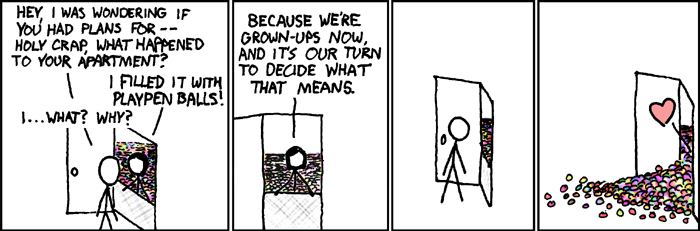
\includegraphics[width=.8\textwidth,keepaspectratio]{img/xkcd/grownups.png}\\
{\footnotesize \textit{I've looked into this, and I can't figure out a way to do it cheaply.\\And I guess it wouldn't be sanitary. (https://xkcd.com/150)}
\end{center}

\pagebreak

\section*{Der Barkhausen-Bau}
Unser Fakultätsgebäude ist zwar schön, kann aber nicht alles bieten, was eine KIF an Anforderungen bereithält.
Wir hab aus diesem Grund etwas Gebäude der Elektrotechniker angemietet.
Mehr oder weniger auf der anderen Straßenseite des APB findet ihr den Barkhausen-Bau.

\subsection*{Plena -- Heinz Schönfeld Hörsaal}
Das Hauptevent der Konferenz sind ohne Zweifen die drei Plena: Erstkiffelplenum, Anfangsplenum und Abschlussplenum.
Sie finden im denkmalgeschützten brandneuen Heinz-Schönfeld-Hörsaal statt.
Der Hörsaal ist der Teil des Barkhausen-Baus, der der Informatikfakultät am nähesten ist.
Über die Straße und ihr seid dort.
Zu beachten ist, dass der Saal mit einer Raumnummer versehen ist, die es eigentlich gar nicht gibt.
% TODO: welche nummer ist das?
Ignoriert diese also einfach.

\subsection*{AK-Räume -- 106, 188, 189, 213, 218}
Die Seminarräume im APB fassen maximal 30 Menschen auf einmal.
Im Barkhausen-Bau gibt es dehalb weitere Räumlichkeiten mit Fassungsvermögen von bis zu 88 Menschen.
Diese weiteren AK-Räume sind so ausgeschildert, dass ihr sie hoffentlich finden werdet.

\section*{Gemeinschaftilche Nahrungsaufnahme}
Neben dem obligatorischen ewigen Frühstück gibt es für euch jeden Tag eine warme Mahlzeit.
Ihr habt bei eurer Anreise eine Mensakarte erhalten, mit der ihr in jeder der Dresdner Mensen bezahlen könnt -- zu studentischen Preisen.
Die Karten sind jeweils mit 10€ aufgeladen die ihr nach Belieben ausgeben könnt.
Ihr seid also in keinster Weise in der Zusammenstellung eurer Mahlzeit eingeschränkt und wenn ihr keine Lust auf eine Hauptspeise habt, ist das auch in Ordnung; Mehr Guthaben für den Nachtisch.
Eine Übersicht des Angebots aller Mensen ist unter \link{https://www.studentenwerk-dresden.de/mensen/speiseplan/} einzusehen.
Ist das Guthaben aufgebraucht, habt ihr die Möglichkeit, die Karte selbst an einer beliebigen Kasse in der Mensa neu aufzuladen.
Die Mensakarte hat ein Pfandwert von 5€, mit dem bereits vor Ankunft eure KdV-Konten belastet wurden.
Bitte gebt die Karten am Ende der Veranstaltung wieder ab.

\subsection*{Alte Mensa}
Ca. 5 Minuten zu Fuß vom APB entfernt erreicht ihr die Alte Mensa, die größte und schönste Mensa der TU\@.
Da sie die nächste Mensa zur Fakultät ist und gleichzeitig auch die meisten Gerichte anbietet, dürfte die selbsternannte \enquote{kulinarische Schlagader im Herzen des Campus} eigentlich all eure Bedürfnisse decken.
Zu Stoßzeiten während der Vorlesungszeit ist die Alte Mensa meist hoffnungslos überfüllt, doch für euch haben wir Ferien bestellt und damit sollte das Erlebnis einer Mahlzeit im Brat$^2$ ohne Frust auskommen.

\subsection*{Mensa U-Boot}
Die Bio-Mensa auf dem Campus setzt sich durch die stilvolle Einrichtung von den anderen Mensen ab, definiert sich aber auch durch die Zutaten aus biologischer und lokaler Erzeugung.
Das in der Mensa U-Boot verwendete Fleisch kommt direkt aus dem Westen Dresdens, was den Preis der Mahlzeiten allerdings nicht unerheblich erhöht.
Wählt ihr die fleischlose Alternative, sollten sich die Preise nicht sonderlich von denen anderer Mensen unterscheiden.
Fußweg ca. 15 Minuten.

\subsection*{Mensa Zeltschlösschen}
Klassische Mensa, die der Alten Mensa in so ziemlich allen Punkten unterlegen ist.
Falls euch das Angebot der Alten Mensa nicht zusagt, könnt ihr den Fußweg von 15 Minuten gern in Kauf nehmen.

\subsection*{Mensa Siedepunkt}
Am anderen Ende des Campus, hinter ca. 20 Minuten Fußweg, liegt der Siede.
% TODO: gibts da wirklich Abendangebot in den Ferien?
Den relativ weiten Weg machen die langen Öffnungszeiten wett, so ist der Siedepunkt die einzige Mensa mit Abendangebot in der vorlesungsfreien Woche.

\subsection*{\enquote{Mensa} Firat}
Ohne Zweifel die beliebteste Mensa auf dem Campus, schenkt man den Aussagen Dresdner FSRlingen glauben, ist Firat.
Es handelt sich hierbei um einen unabhängigen Dönerladen, doch durch den effizienten Umgang mit überdurchschnittlich hohem studentischen Andrang wird er gern auch scherzhaft als Mensa bezeichnet.
Das Dönerhaus liegt knapp 10 Minuten Fußweg vom APB entfernt und lockt mit guter Qualität, gemütlichem Ambiente und einer vergleichsweise großen Auswahl an Gerichten.

\subsection*{Samstag -- Grillen}
Da die meisten Mensen leider kein Wochenendangebot anbieten, haben wir für Samstag sämtliche an der TU-Dresden ausleihbare Grills organisiert.
Zur Mittagszeit wird es auf dem Parkplatz also ein riesiges BBQ geben.


\subsection*{Massenvernichtungswaffel}
Am Infopoint wird es außerdem Zugriff auf die Massenvernichtungswaffel geben.
Dabei handelt es sich um eine Ausrüstung zur Waffelzubereitung, die dafür gedacht ist, zu jeder beliebigen Zeit Waffeln für alle anwesenden KIFfel zu machen.
Fragt bei Waffelheißhunger also einfach am Infopoint nach der Massenvernichtungswaffel und beginnt mit der Zubereitung.
